\begin{appendices}
\addtocontents{toc}{\protect\setcounter{tocdepth}{0}}

\chapter{Algorithms}
\label{appendix:algorithms}
Here, we list all of the infector algorithms of this thesis that have been proven to produce correct results and be faster than the original approaches.

\section{All-to-All}
These algorithms are designed to calculate contacts and transmissions between all members of a pool. 

\subsection{Original}
Section \ref{subsec:contacts_and_transmissions}, page \pageref{subsec:contacts_and_transmissions}.
\\\\
\textbf{Description:} Double iteration over the members of a pool to match everyone with each other. For every pair of individuals a contact probability is calculated to determine whether they have contact or not. If contact has been made and one of them is susceptible and the other infectious, a transmission probability is calculated to determine if the susceptible one gets infected
\\\\
\textbf{Implementation:} Algorithm \ref{alg:all-to-all}, page \pageref{alg:all-to-all}.

\subsection{Iterative-intervals}
Section \ref{sec:iterative_intervals}, page \pageref{sec:iterative_intervals}.
\\\\
\textbf{Description:} Divides the members of a pool in age intervals in which everyone has the same contact rate, except for household pools that use the original approach. Calculate the contact probability for every pair of intervals only once. Then iterates over the intervals to match every interval with another, including an interval with itself. When we match an interval with itself, for every pair of individuals between two intervals, determine if there is contact based on the previously calculated contact probability. If there is contact, register this and determine if there is transmission as before.
\\\\
\textbf{Implementation:} Algorithm \ref{alg:iterative_intervals}, page \pageref{alg:iterative_intervals}.

\subsection{Sampling-with-iteration}
Section \ref{sec:sampling_with_iteration}, page \pageref{sec:sampling_with_iteration}.
\\\\
\textbf{Description:} Sort the members of a pool in age intervals and iterate over all the intervals as before and calculate the contact probabilities. When we match an interval with itself, use the \textsc{Iterative-intervals} algorithm. When we match two different intervals with each other, iterate over the members of the first interval. For every iterated member, calculate the sample size with a binomial distribution based on the contact probability and the size of the second interval. Then, randomly select that amount of members of the second interval and register contact with all of them and handle transmissions as before.
\\\\
\textbf{Implementation:} Algorithm \ref{alg:sampling_with_iteration}, page \pageref{alg:sampling_with_iteration}.

\subsection{Full-sampling (>150)}
\textsc{Full-sampling}: Section \ref{sec:full_sampling}, page \pageref{sec:full_sampling}.
\\\\
\textsc{Full-sampling (>150)}: Section \ref{sec:adjusted_full_sampling}, page \pageref{sec:adjusted_full_sampling}.
\\\\
\textbf{Description:} Same as \textsc{Sampling-with-iteration}, except for handling contacts between members of the same interval. When we match an interval with itself, calculate a special contact probability so we can iterate over the members to calculate a sample size based on the entire interval. Then proceed as we did before in \textsc{Sampling-with-iteration}. Because we do not take into account that there are duplicate contacts when sampling in the same interval, the results are incorrect due to double probability of transmission for a duplicate contact. To reduce the probability for duplicate contacts, we adjusted the algorithm so it is only used on pools with at least 150 people, the other pools use the original algorithm.
\\\\
\textbf{Implementation:} Algorithm \ref{alg:full_sampling}, page \pageref{alg:full_sampling}.

\subsection{Full-sampling-unique-contacts (>150)}
Section \ref{sec:full_sampling_unique_contacts}, page \pageref{sec:full_sampling_unique_contacts}.
\\\\
\textbf{Description:} Continue on the \textsc{Full-sampling} algorithm, with an adjustment to sampling in the same interval. Create a hash set to store all the contacts instead of registering them and handling the transmission. Because it is a set, we do not need to worry about duplicate contacts since sets cannot contain duplicate values. After sampling all the contacts, iterate over the hash set and register every contact and handle the transmissions as before.
\\\\
\textbf{Implementation:} Algorithm \ref{alg:full_sampling_unique_contacts}, page \pageref{alg:full_sampling_unique_contacts}, with the adjustment that we only use the algorithm for pools with at least 150 people.

\section{Inf-to-Sus}
These algorithms are designed to only calculate transmissions between the infectious and susceptible members of a pool.

\subsection{Original}
Section \ref{subsec:contacts_and_transmissions}, page \pageref{subsec:contacts_and_transmissions}.
\\\\
\textbf{Description:} Sort the members of a pool according to their health status and stop the algorithm if there are no members infectious. Otherwise, iterate over every infectious person and match them with every susceptible one. Calculate the contact probability for every pair and the transmission probability. Combine these probabilities to determine whether there is contact and transmission or not, and infect the susceptible one if there is.
\\\\
\textbf{Implementation:} Algorithm \ref{alg:inf-to-sus}, page \pageref{alg:inf-to-sus}.

\subsection{Iterative-intervals (sort sus)}
Section \ref{subsec:iterative_intervals_inf-to-sus}, page \pageref{subsec:iterative_intervals_inf-to-sus}.
\\\\
\textbf{Description:} Sort the members of a pool based on their health status as before, then sort the susceptible members in age intervals. Iterate over the infectious members and the susceptible intervals, and calculate the contact and transmission probabilities for every pair of an infectious member and susceptible interval. Iterate over the susceptible interval members and determine if there is contact and transmission based on the previously combined probability.
\\\\
\textbf{Implementation:} There is no explicit algorithm implementation presented, but it can be derived from the original \textsc{Inf-to-Sus} (Algorithm \ref{alg:inf-to-sus}, page \pageref{alg:inf-to-sus}) and \textsc{Iterative-intervals} (Algorithm \ref{alg:iterative_intervals}, page \pageref{alg:iterative_intervals}) algorithms.

\chapter{Configurations}
\label{appendix:configurations}

\begin{table}
\centering
\begin{tabular}{@{}lll@{}}
\toprule
Parameter & Value & Additional info \\ \midrule
age\_contact\_matrix\_file & \begin{tabular}[t]{@{}l@{}}contact\_matrix\_flanders\\ \_conditional\_teachers.xml\end{tabular} &  \\
event\_log\_level & 'All' or 'Transmissions' & \begin{tabular}[t]{@{}l@{}}respectively for all-to-all\\ and inf-to-sus\end{tabular} \\
event\_output\_file & false &  \\
disease\_config\_file & disease\_covid19\_age.xml &  \\
global\_information\_policy & NoGlobalInformation &  \\
holidays\_file & holidays\_none.csv & \begin{tabular}[t]{@{}l@{}}adjusted so that contact\\ tracing occurs every day\end{tabular} \\
immunity\_profile & None &  \\
immunity\_rate & 0.8 &  \\
num\_days & 100 &  \\
num\_participants\_survey & 10 &  \\
num\_threads & 1 &  \\
output\_cases & true &  \\
output\_persons & false &  \\
output\_summary & false &  \\
population\_file & \begin{tabular}[t]{@{}l@{}}pop\_belgium11M\_c500\\ \_teachers\_censushh.csv\end{tabular} &  \\
population\_type & default &  \\
rng\_seed & 2020 &  \\
r0 & 11 &  \\
seeding\_age\_max & 99 &  \\
seeding\_age\_min & 1 &  \\
num\_infected\_seeds & 1200 &  \\
start\_date & 2020-03-02 &  \\
stride\_log\_level & info &  \\
track\_index\_case & false &  \\
vaccine\_link\_probability & 0 &  \\
vaccine\_profile & Random &  \\
vaccine\_rate & 0.8 &  \\
detection\_probability & 0.5 &  \\ \bottomrule
\end{tabular}
\caption{Configurations to run general Stride simulations throughout this thesis.}
\label{tab:configurations}
\end{table}

\chapter{Sampling same interval}
\label{appendix:sampling_same_interval}
The following pages present the reasoning and prove for sampling in the same interval, for which all credit is due to prof. dr. Stijn Vansummeren.
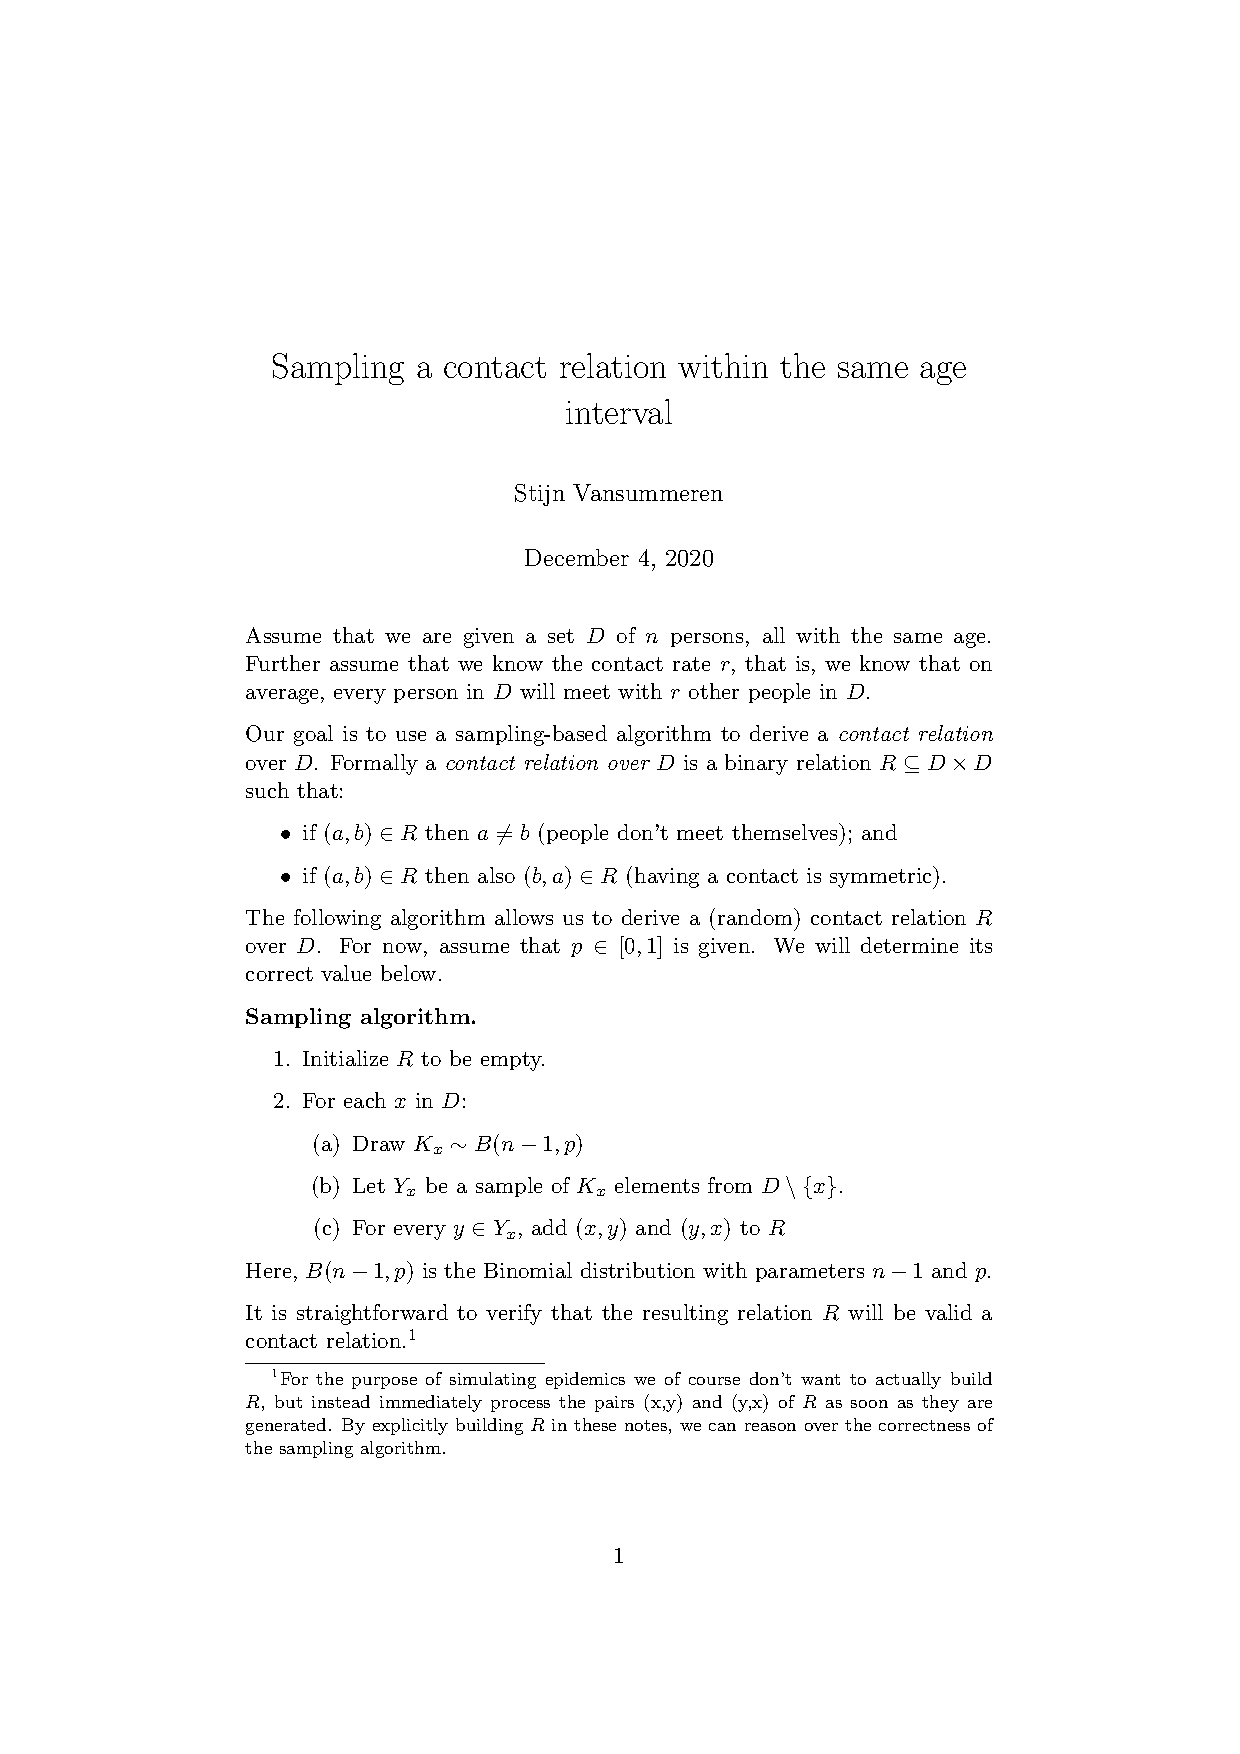
\includepdf[scale=.9,pages=-,pagecommand={}]{Appendix/sampling_same_interval.pdf}

\chapter{Een hoogperformante toolkit om infectieziektes te modelleren: Nederlandse samenvatting}
Wanneer een ziekte opduikt is het van cruciaal belang om deze te onderzoeken zodat we ze kunnen bestrijden. Dergelijke onderzoeksprocessen vergen zeer veel werk en tijd om de ziekte volledig te doorgronden. Tijdens de COVID-19 pandemie werden er voortdurend nieuwe maatregelen getroffen, door onder andere de WGO (Wereldgezondheidsorganisatie) en regeringen, om deze infectieziekte onder controle te houden. Om zulke maatregelen te nemen baseert men zich op de kennis en data die voorhanden is op dat moment. Deze informatie kan voortkomen uit allerlei verschillende hoeken waaronder klinische onderzoeken, maar ook computersimulaties die gebruik maken van computermodellen om voorspellingen te maken over hoe de ziekte zal voortbewegen door een populatie. Elke simulatie maakt gebruik van verscheidene parameters die beschrijven hoe deze uitgevoerd moet worden om zo verschillende situaties te creëren. Zulke parameters beschrijven onder andere hoe gemakkelijk een ziekte kan worden overgedragen, hoelang men ziek blijft, wanneer de scholen sluiten, etc. Door deze waarden telkens te veranderen kan men heel veel verschillende simulaties uitvoeren en dus ook veel verschillende situaties nabootsen. Hierdoor kan men allerlei verschillende inzichten verkrijgen in wat de gevolgen kunnen zijn voor de maatregelen. Hoe meer verschillende simulaties men kan uitvoeren, hoe meer inzichten men kan verwerven en dus ook hoe beter men een zicht krijgt in de maatregelen waardoor men uiteindelijk beter kan inspelen op de ziekte. Om deze simulaties zo accuraat mogelijk te maken, maakt men gebruik van representatieve populaties zoals de bevolking van België die elf miljoen bewoners telt. Dit is zeer veel data om te behandelen, wat maakt dat de simulaties behoorlijk veel tijd en middelen in beslag kunnen nemen. Het doel van deze thesis is om een dergelijk computermodel, namelijk Stride, te verbeteren zodat er sneller en makkelijker resultaten geproduceerd kunnen worden. Deze verbeteringen uiten zich in twee onderdelen:
\begin{enumerate}
    \item Het model optimaliseren zodat de berekeningen tijdens een simulatie sneller uitgevoerd kunnen worden. Zoals gezegd, zorgt dit ervoor dat er meer simulaties uitgevoerd kunnen worden waardoor er dus meer en betere inzichten kunnen verkregen worden.
    \item Er is enige kennis vereist van hoe Stride berekeningen doet om er simulaties mee te kunnen uitvoeren. In deze thesis bieden we een DSL (domain specific language oftewel domeinspecifieke taal) aan om het gebruik van Stride te abstraheren, wat ervoor zorgt dat er makkelijker met het model kan gewerkt worden. Door enkele regels te declareren in deze taal wordt er achterliggend bepaald hoe de simulatie dient te worden uitgevoerd.
\end{enumerate}

\section{Infectieziektes modelleren}
Vooraleer we verder gaan met Stride, hebben we enige voorkennis nodig van infectieziektes en hoe deze gemodelleerd kunnen worden.

\subsection{Concepten van infectieziektes}
Een infectieziekte wordt altijd veroorzaakt door een ziekteverwekker, zoals een virus of bacterie. Bij het modelleren hiervan wordt er vooral gefocust op ziektes waarvan de verwekkers kunnen worden overgedragen via contact tussen personen. Wanneer zo een transmissie van een ziekteverwekker gebeurt van de ene persoon naar de andere, start bij de ontvanger een nieuw infectie proces. Hoe dit eruit ziet is verschillend voor elk proces en hangt af van allerlei factoren zoals de gezondheid van de persoon, de karakteristieken van de ziekte, etc. Er zijn verschillende stadia die kunnen voorkomen in zo een proces. Wanneer iemand is blootgesteld aan een ziekteverwekker, begint de incubatie fase waarin hij nog geen symptomen heeft. Vanaf dat dit wél het geval is, start de symptomatische periode die blijft duren totdat alle symptomen verdwenen zijn. Bij de de start van het proces is men ook nog niet meteen besmettelijk, dit heet de latente periode. Vanaf dat dit verandert start de besmettelijke periode die duurt zolang dat men nog iemand anders kan besmetten. Hoelang deze fasen duren is afhankelijk van de persoon en ziekte. Wanneer de fasen met betrekking tot symptomen en deze met betrekking tot besmetting niet gelijk lopen, zegt men dat iemand asymptomatisch is. Het is ook mogelijk dat iemand immuun is voor de ziekte, wat betekent dat hij geen symptomen zal vertonen en mogelijks ook niet besmettelijk is.

\subsection{Modellen}
Deze concepten kunnen vervolgens gebruikt worden om modellen te creëren voor infectieziektes. De meest eenvoudige zijn de wiskundige modellen die een bepaalde populatie indelen op basis van hun gezondheidsstatus: vatbaar, blootgesteld, besmettelijk en genezen. Deze worden al decennia lang gebruikt om snel een overzicht te krijgen van hoe een ziekte zal evolueren. Aangezien dat computers tegenwoordig krachtige machines zijn, worden deze ingezet om ziektes gedetailleerder voor te kunnen stellen. Het bouwen van computermodellen voor zulke dingen kan op zeer veel manieren gebeuren afhankelijk van wat ze moeten berekenen en produceren. De architectuur van Stride is gebaseerd op het agent-based model, waarin een populatie wordt voorgesteld als allemaal verschillende individuen. In zulke modellen worden interacties tussen individu's berekend om zo een beeld te krijgen van hoe een ziekte voortbeweegt.

\section{Stride}
Het computermodel waar deze thesis zich op focust, Stride, is gebaseerd op drie kernprincipes om zo accuraat mogelijk een infectieziekte te simuleren: leeftijd, type dag, en sociale context. Ieder individu heeft een bepaalde leeftijd die gebruikt wordt voor alle berekeningen. Hiermee wordt bepaald hoe personen met elkaar interageren, omdat mensen meer geneigd zijn contact te hebben met leeftijdsgenoten dan met personen die vijftig jaar ouder zijn. Wat voor soort dag gesimuleerd wordt heeft ook een zeer grote invloed op het gedrag van een populatie, aangezien bijvoorbeeld mensen geen contact hebben met collega's in het weekend of op een feestdag. De sociale context is ook belangrijke factor om te bepalen hoe mensen met elkaar omgaan, aangezien mensen in hetzelfde huishouden veel meer contact hebben met elkaar dan met hun collega's op het werk.

\subsection{Structuur}
Zoals eerder vermeld stelt Stride een populatie voor aan de hand van individuen. Deze bevatten verscheidene eigenschappen zoals hun leeftijd en gezondheid. De gezondheid van een persoon is voor iedereen verschillend en wordt gedefinieerd aan de hand van enkele kenmerken. Een eerste kenmerk is de status, wat gebaseerd is op de wiskundige modellen, en kan zowel vatbaar, blootgesteld, besmettelijk, genezen, en immuun. Andere kenmerken bepalen de eigenschappen van iemands gezondheid zoals hoe lang de fases van een infectie duren. Om te bepalen wie met elkaar contact zal hebben, wordt iedereen ingedeeld in \textit{contact pools}. Enkel binnen zo een pool is het mogelijk voor individu's om contact met elkaar te hebben. Er zijn vier soorten pools: huishouden, primaire gemeenschap, secundaire gemeenschap en de dagdagelijkse bezigheid. Het huishouden spreekt voor zich, waarin het ook mogelijk is om iedere dag contact met anderen te hebben. De primaire en secundaire gemeenschappen zijn niet specifiek te beschrijven, maar stellen de mensen voor die men kan ontmoeten in de vrije tijd zoals bij hobby's, vrienden, etc. De primaire gemeenschap is in het algemeen enkel actief in het weekend of feestdagen en de secundaire enkel tijdens doordeweekse dagen. Voor de dagdagelijkse bezigheid pools zijn er drie onderverdelingen: werk, K-12 school (wat alle onderwijsinstellingen voor kinderen jonger dan 18 jaar voorstelt) en college (wat alle onderwijsinstellingen voor jongvolwassenen voorstelt tussen 18 en 23 jaar). Elk individu is lid van exact één huishouden, primaire gemeenschap en secundaire gemeenschap en men kan ook lid zijn van één of geen dagdagelijkse bezigheid pool. Leerkrachten en proffen zijn behoren tot een K-12 school of college pool, aangezien ze contact hebben met hun leerlingen.

\subsection{Configuraties}
Het Stride model is gebouwd zodat er veel verschillende simulaties mee uitgevoerd kunnen worden. Dit is mogelijk door allerlei parameters die kunnen worden ingesteld via de configuraties, zoals hoe de populatie eruit ziet. Ook kan een kalender ingesteld worden die info bevat over speciale dagen zoals feestdagen, schoolvakanties, de dagen waarop social distancing actief is, etc. De eigenschappen van de ziekte kunnen ingesteld worden, zodat allerlei verschillende soorten kunnen gesimuleerd worden of bijvoorbeeld dezelfde ziekte met iets andere besmettingswaarden. De contact vectors moeten ook geconfigureerd worden, want deze representeren hoeveel contacten een individu gemiddeld heeft per dag afhankelijk van zijn leeftijd en het type pool. Buiten enkele numerieke waarden is er ook nog de mogelijkheid om te kiezen welke info geproduceerd moet worden. Dit kan enkel de transmissies zijn gedurende de simulatie, maar ook dat alle contacten eveneens bijgehouden moeten worden wat een grote invloed heeft op hoe de simulatie verloopt.

\subsection{Simulatie}
In het algemeen kunnen we Stride opdelen in twee onderdelen, namelijk de initialisatie en het daadwerkelijk simuleren aan de hand van berekeningen. Het initialiseren gebeurt vanzelfsprekend in het begin en zet de simulatie klaar door onder andere de populatie te creëren naargelang de configuraties en willekeurig mensen selecteren die geïnfecteerd starten. Hierna begint Stride de dagen te simuleren die allemaal bestaan uit dezelfde drie fases. Als eerste start een dag met het updaten van alle individuen, wat inhoudt dat hun gezondheid bijvoorbeeld vordert van besmettelijk naar genezen, maar ook in welke pools de persoon actief gaat zijn de komende dag. Hierna is er een mogelijkheid om contact tracing uit te voeren, maar dit is een optionele feature en heeft geen grote impact op de simulaties. Als laatste van de dag worden alle berekeningen gedaan om te kijken wie met elkaar contact heeft en wie besmet wordt. Hiervoor zijn er twee 'infector' algoritmes die gebruikt kunnen worden afhankelijk van welke data de simulatie moet voortbrengen. Alle pools van elk type worden één voor één overlopen en behandeld in zo een algoritme.

\subsubsection{All-to-all}
Het eerste algoritme, genaamd \textit{all-to-all}, gaat iedereen die aanwezig is binnenin een pool paarsgewijs met elkaar vergelijken. Per paar wordt een contactprobabiliteit berekend die we gebruiken om willekeurig te bepalen als er contact is tussen de twee. Indien er contact is wordt dit geregistreerd en checken we als één van de twee besmettelijk is en de andere vatbaar. Als dit het geval is wordt de kans op transmissie berekend die we ook gebruiken om willekeurig te beslissen als de ander besmet wordt.

\subsubsection{Inf-to-sus}
De tweede infector methode gaat enkel besmettelijke personen van een pool paarsgewijs vergelijken met alle vatbare mensen, mits ze beide aanwezig zijn, en noemen we het \textit{inf-to-sus} algoritme. Hiermee worden enkel de noodzakelijke berekeningen gedaan om te bepalen wie geïnfecteerd raakt. Per paar wordt de totale kans op contact én transmissie berekend om willekeurig te bepalen als er een besmetting gebeurt. Om gestructureerd deze methode toe te kunnen passen, worden de pools in het begin van het algoritme gesorteerd op basis van hun gezondheidsstatus. Als hieruit blijkt dat er geen besmettelijke personen in een pool zitten, zijn er geen berekeningen nodig en stopt het algoritme vroegtijdig om geen onnodige tijd te verspillen.

\subsubsection{Kansen berekenen}
Zoals vermeld gebruikt ons model kansberekeningen om willekeurig te bepalen wie contact heeft en wie besmet raakt. Per individu paar wordt een functie gebruikt om de kans op contact tussen de twee te berekenen. Deze maakt gebruik van de contact vectoren en de leeftijden van beide om de berekeningen uit te voeren rekening houdend met nog enkele andere kleine factoren. De functie die de kans op transmissie berekent, kijkt naar de eigenschappen van de ziekte alsook als de overdrager asymptomatisch is en als de ontvanger jonger is dan 18.

\subsection{Data}
Om betere inzichten te verwerven is het ook belangrijk om te weten hoe de data eruit ziet die we gebruiken in de simulaties. We hebben eerder vermeld dat Stride voornamelijk gebruikt wordt voor de Belgische bevolking na te bootsen, wat ervoor zorgt dat de populatie in de simulaties bestaat uit elf miljoen verschillende individuen. Verder kijken we naar de contact pool types en hoe deze verdeeld zijn, wat voorgesteld wordt in Tabel \ref{tab:contact_pools_statistics}. Hieruit leren we dus dat er bijna vijf miljoen huishoudens zijn in tegenstelling tot beide gemeenschappen waarvan er voor elk slechts 22 000 pools zijn. Het is ook opmerkelijk dat de grootte van een huishouden ligt tussen 1 en 6 personen, terwijl de gemeenschappen ongeveer 50 tot 1430 mensen kunnen bevatten. Er zijn ongeveer 566 000 werk pools die 1 tot 1000 leden kunnen bevatten, alhoewel de verdeling van de groottes laat zien dat 94\% van de werk pools maximum 9 leden heeft zoals te zien is in Figuur \ref{fig:workplace_poolsize_ranges}. De scholen bevatten nooit meer dan 50 leden waardoor ze dus ook relatief klein zijn.

\subsection{Analyse}
Als we Stride willen optimaliseren, moeten we weten waar de pijnpunten liggen door het model grondig te analyseren. Als eerste valt op dat er een mogelijkheid is om parallellisatie toe te passen met OpenMP, wat gebruik maakt van multithreading, voor het updaten van individuen en voor het toepassen van de infector algoritmes op de pools. Vervolgens meten we de performance van Stride simulaties met beide infector algoritmes en kijken we naar hoeveel tijd de drie fases per dag in beslag nemen. Tabel \ref{tab:basis_runtime_stats} toont dat all-to-all bijna alle tijd spendeert aan het berekenen van de contacten en transmissies, terwijl inf-to-sus meer dan zeventig keer sneller is voor het infector gedeelte. Inf-to-sus is in totaal dertig keer sneller dan all-to-all en heeft hoogstwaarschijnlijk weinig ruimte voor verbetering. Wanneer we simulaties uitvoeren met behulp van parallellisatie, zien we dat de het juist langer duurt en dus het tegenovergestelde effect heeft.

\section{Eerste optimalisatie}
Tijdens het analyseren viel op dat de functie voor het berekenen van de contactprobabiliteiten het meeste tijd in beslag nam per dag. Na het onderzoeken van de oorzaak bleek dat deze functie sub-optimaal geïmplementeerd was. Een parameter van deze functie is een pointer naar de gehele populatie in de vorm van een \textit{std::shared\_pointer}. Deze werd echter doorgegeven door middel van pass-by-value, waardoor het achterliggend systeem van de shared pointer telkens een teller moet updaten. Dit kost een zeer klein beetje tijd meer, maar het all-to-all algoritme vergelijkt iedereen binnen een pool met elkaar en berekent daarvoor de contactprobabiliteit. Dit zorgt ervoor dat die extra kost ontelbaar keer erbij komt per dag en dus uiteindelijk voor een grote overhead zorgt. Het updaten van de teller is tevens een atomaire operatie, wat ervoor zorgt dat slechts één thread dit kan uitvoeren terwijl alle andere moeten wachten op hun beurt vooraleer ze verder kunnen naar de functie. Dit is ook de reden dat multithreading het tegenovergestelde effect heeft.
\\\\
We hebben dit opgelost door de shared pointer van de populatie via pass-by-reference mee te geven. Hierdoor werd de dagelijkse tijd voor de infector van all-to-all gemiddeld 1,83 keer sneller en de totale dagelijkse tijd 1,81. De infector van inf-to-sus werd 1,09 keer versneld waardoor de totale tijd 1,04 keer sneller is. Dit loste eveneens het probleem van multithreading op, waardoor parallellisatie nu daadwerkelijk ervoor zorgt dat een simulatie sneller verloopt. Voortaan, als we naar het origineel all-to-all algoritme verwijzen, gaat het over deze geoptimaliseerde versie.

\section{Samplen}
Omdat het inf-to-sus algoritme weinig ruimte biedt voor verbetering, focussen we enkel nog op all-to-all voor het optimaliseren. Meeste Stride simulaties verlopen zonder parallellisatie, dus wordt er ook enkel uitgebreid getest op simulaties met één thread. All-to-all vergelijkt iedereen een pool met elkaar, waardoor het algoritme een tijdscomplexiteit $\mathcal{O}(n^{2})$ heeft waarin $n$ staat voor het aantal mensen in de pool. Dit zorgt ervoor dat het algoritme kwadratisch keer meer tijd in beslag neemt naarmate de pools groter worden. Om dit op te lossen willen we per persoon een sample nemen uit de pool waar hij contact mee zal hebben i.p.v. deze te moeten vergelijken met iedereen. In theorie zou dit ongeveer een lineaire tijdscomplexiteit moeten hebben in functie van de pool grootte. Dit willen we implementeren met behulp van een binomiale distributie om de sample groottes te berekenen. Hiervoor is echter een contactprobabiliteit nodig die geldig is voor een persoon met iedereen waaruit het sample getrokken wordt, maar de contact verhoudingen zijn verschillend afhankelijk van de leeftijd.

\subsection{Iteratieve intervallen}
Het bovenvermelde probleem lossen we op door de leden van een pool op te splitsen in leeftijdsintervallen, zodat iedereen in een interval dezelfde waarden heeft in de contact vector. Dit leidt tevens ook al tot de eerste optimalisatie, aangezien we nu alle personen uit twee intervallen met elkaar kunnen vergelijken en maar één contactprobabiliteit hiervoor moeten berekenen. Het nieuwe algoritme itereert over de intervallen en per interval-paar itereert het vervolgens over alle mogelijk individu paren, waardoor we dit de \textit{iteratieve intervallen} methode noemen. Omdat de kans op contact binnen een huishouden altijd 0,999 is, passen we dit toe op alle pools behalve de huishoudens. Deze aanpak blijkt correcte resultaten te produceren en zorgt voor opmerkelijke tijdswinsten door enkel het aantal keer dat de kans moet berekend worden te verminderen. Het levert een dagelijks gemiddelde infector tijd op die 1,85 keer sneller is dan het origineel en 1,80 keer sneller is voor een totale dag. In het algemeen nemen de gemeenschappen veruit het meeste tijd in beslag, wat te wijten is aan de grootte die ze kunnen hebben. De tijdswinst is daardoor ook voornamelijk te danken aan deze pools die nu veel minder tijd nodig hebben.

\subsection{Samplen met iteratie}
De techniek van iterative intervallen kunnen we nu gebruiken om een algoritme te creëren dat gebruikt maakt van samplen. Per intervalpaar berekenen we een contactprobabiliteit die we gebruiken in een binomiale distributie op basis van de grootte van een interval. Vervolgens itereren we over alle leden van het ene interval en berekenen we een sample grootte $k$ per persoon door middel van de binomiale distributie. Hierna selecteren we willekeurig $k$ personen uit het andere interval waarvoor er dan contact gemaakt wordt en eventueel ook transmissie. Het probleem aan deze aanpak is dat het vergelijken van mensen in hetzelfde interval niet mogelijk is op deze manier. Dit lossen we op door de mensen in eenzelfde interval nog steeds allemaal met elkaar te vergelijken, waardoor het de naam \textit{samplen met iteratie} krijgt. Deze nieuwe aanpak produceert correcte resultaten en merkbare tijdwinsten. De infector is hierdoor 2,63 keer sneller dan het origineel en een totale dag 2,50 keer. Wat opvalt is dat de werk pools geen tijdswinst hebben ten opzichte van iteratieve intervallen. Dit komt doordat de werk pools slechts in drie intervallen opgesplitst worden waarvan er eentje bijna alle leden bevat, wat ervoor zorgt dat ze nog steeds gelijkaardig werken aan iteratieve intervallen.

\subsection{Volledig samplen}
Het voorval van de werk pools willen nu oplossen zodat we ook deze pool types optimaliseren. Deze nieuwe methode gaat verder op samplen met iteratie en past enkel aan hoe we de contacten binnen eenzelfde interval bepalen. Hiervoor berekenen we de contactprobabiliteit op een andere manier wanneer we binnen eenzelfde interval contacten willen bepalen. Met deze nieuwe probabiliteit kunnen we itereren over alle personen in een interval en telkens een sample grootte berekenen op basis van het hele interval. Het is nu wel mogelijk dat een contact tussen twee individuen twee keer voorkomt, wat ervoor zorgt dat er dan een 'extra' mogelijkheid is voor transmissie. Uit de testen blijkt ook dat dit niet de juiste resultaten teruggeeft, omdat de ziekte meer verspreid kan worden wanneer een duplicate contact optreedt. De oplossing hiervoor is om enkel relatief grote pools dit algoritme te laten gebruiken, zodat de kans op duplicate contacten zeer klein is. Hiervoor zetten we de threshold op 150, wat dus betekent dat pools met minder dan 150 personen het origineel algoritme gebruiken en de rest volledig samplen. Dit geeft wel accurate resultaten terug en heeft, zoals we voorspelden, de snelste tijden naarmate een pool groter wordt. Deze aanpak heeft een speedup van 2,84 voor de gemiddelde infector en 2,67 voor een totale dag. In Figuur \ref{fig:fs_pSize_vs_rest_type_totals} zien we dat op deze manier de gemeenschappen en werkplekken nog steeds de beste tijd hebben, en dat de andere pool types amper tijdsverlies hebben.

\subsection{Volledig samplen van unieke contacten}
Omdat we met volledig samplen niet 100\% correcte resultaten hebben door het samplen in hetzelfde interval, hebben we het algoritme aangepast om enkel unieke contacten te behandelen. Dit doen we door alle contacten op te slaan in een hash set zonder ze te registreren of transmissies verder af te handelen. Op het einde van samplen in hetzelfde interval, overlopen we onze hash set om alle contacten te registreren en transmissies te berekenen. Omdat we gebruik maken van een set, moeten we niet extra checken als een contact al voorkomt aangezien een set geen duplicate waarden kan bevatten. Opgelet, dit geldt enkel voor het samplen in hetzelfde interval, twee verschillende intervallen worden behandeld zoals in samplen met iteratie. Dit algoritme produceert correcte resultaten, zelfs voor de kleinste pools. De extra overhead door de unieke contacten te verzekeren zorgt er wel voor dat dit algoritme geen geweldige tijden neerzet. In vergelijking met het origineel is dit algoritme slechts 2,36 keer sneller voor de infector en 2,27 keer sneller voor een totale dag. Volledig samplen (>150) en samplen met iteratie doen het dus beter dan volledig samplen van unieke contacten.

\subsection{Inf-to-sus}
Deze optimalisaties willen we uiteraard ook testen op het inf-to-sus algoritme om te kijken als we betere tijden kunnen verwezenlijken. Om dit te doen werken moeten we zowel de besmettelijke personen als de vatbare in leeftijdsintervallen verdelen. Aangezien er meestal weinig besmettelijke personen aanwezig zijn in een pool, creëren we ook een algoritme dat deze personen niet sorteert in intervallen en dus er gewoon over itereert. De iteratieve intervallen methode 
waar we enkel de vatbare mensen sorteren is het enige algoritme dat correcte resultaten produceert en sneller is dan het origineel. Deze methode is 1,11 keer sneller voor de infector en 1,09 keer sneller voor een totale dag dan het originele algoritme.

\section{Domeinspecifieke taal}
De tweede manier waarop we Stride willen verbeteren is door het gebruiksgemak te verhogen door middel van een domeinspecifieke taal die we EpiQL noemen. Met deze taal kan een gebruiker aan de hand van declaratieve regels beschrijven hoe een Stride simulatie zou moeten werken. Dit zorgt ervoor dat de gebruiker geen gedetailleerde kennis nodig heeft van hoe het achterliggend model werkt. Ook kan dit ervoor zorgen dat we onze besproken optimalisaties kunnen doorvoeren en bepalen welke methode er gebruikt moet worden zonder manuele tussenkomst. Om onze taal te kunnen gebruiken, moeten we een compiler schrijven die een EpiQL programma kan omzetten naar uitvoerbare code. Deze compiler is op het einde van de thesis niet volledig af en er kan dus ook geen demonstratie van gegeven worden. We hebben in de thesis enkel de theorie achter EpiQL uitgelegd alsook de delen van de compiler die geïmplementeerd zijn en welke nog niet. We kozen ervoor om de compiler in Rust te maken, omdat deze taal voordelen heeft zoals een zero-cost abstraction en borrow checker wat resulteert in snelle en veilige code. Aangezien er geen voorgaande kennis over Rust was, moest deze taal ook nog volledig geleerd worden gedurende de thesis.

\section{Conclusie}
We stellen vast dat we sinds de start van deze thesis \textsc{All-to-All} simulaties meer dan vier keer sneller kunnen uitvoeren en zelfs snellere runtimes verwezenlijken voor \textsc{Inf-to-Sus} simulaties. De DSL die we gecreëerd hebben laat ons toe, in theorie, om simulaties uit te voeren zonder uitgebreide kennis te hebben van het model. Een nieuwe masterthesis gaat volgend academiejaar verder op deze, waardoor opvolging voor de DSL is verzekerd. Uiteindelijk concluderen we dat we erin geslaagd zijn Stride te optimaliseren qua snelheid, en dat we een grote aanzet hebben gegeven voor het gebruiksgemak te verbeteren door middel van onze DSL, EpiQL.

\end{appendices}